% Options for packages loaded elsewhere
\PassOptionsToPackage{unicode}{hyperref}
\PassOptionsToPackage{hyphens}{url}
%
\documentclass[
]{article}
\usepackage{amsmath,amssymb}
\usepackage{lmodern}
\usepackage{ifxetex,ifluatex}
\ifnum 0\ifxetex 1\fi\ifluatex 1\fi=0 % if pdftex
  \usepackage[T1]{fontenc}
  \usepackage[utf8]{inputenc}
  \usepackage{textcomp} % provide euro and other symbols
\else % if luatex or xetex
  \usepackage{unicode-math}
  \defaultfontfeatures{Scale=MatchLowercase}
  \defaultfontfeatures[\rmfamily]{Ligatures=TeX,Scale=1}
\fi
% Use upquote if available, for straight quotes in verbatim environments
\IfFileExists{upquote.sty}{\usepackage{upquote}}{}
\IfFileExists{microtype.sty}{% use microtype if available
  \usepackage[]{microtype}
  \UseMicrotypeSet[protrusion]{basicmath} % disable protrusion for tt fonts
}{}
\makeatletter
\@ifundefined{KOMAClassName}{% if non-KOMA class
  \IfFileExists{parskip.sty}{%
    \usepackage{parskip}
  }{% else
    \setlength{\parindent}{0pt}
    \setlength{\parskip}{6pt plus 2pt minus 1pt}}
}{% if KOMA class
  \KOMAoptions{parskip=half}}
\makeatother
\usepackage{xcolor}
\IfFileExists{xurl.sty}{\usepackage{xurl}}{} % add URL line breaks if available
\IfFileExists{bookmark.sty}{\usepackage{bookmark}}{\usepackage{hyperref}}
\hypersetup{
  hidelinks,
  pdfcreator={LaTeX via pandoc}}
\urlstyle{same} % disable monospaced font for URLs
\usepackage{graphicx}
\makeatletter
\def\maxwidth{\ifdim\Gin@nat@width>\linewidth\linewidth\else\Gin@nat@width\fi}
\def\maxheight{\ifdim\Gin@nat@height>\textheight\textheight\else\Gin@nat@height\fi}
\makeatother
% Scale images if necessary, so that they will not overflow the page
% margins by default, and it is still possible to overwrite the defaults
% using explicit options in \includegraphics[width, height, ...]{}
\setkeys{Gin}{width=\maxwidth,height=\maxheight,keepaspectratio}
% Set default figure placement to htbp
\makeatletter
\def\fps@figure{htbp}
\makeatother
\setlength{\emergencystretch}{3em} % prevent overfull lines
\providecommand{\tightlist}{%
  \setlength{\itemsep}{0pt}\setlength{\parskip}{0pt}}
\setcounter{secnumdepth}{-\maxdimen} % remove section numbering
\ifluatex
  \usepackage{selnolig}  % disable illegal ligatures
\fi

\author{}
\date{}

\begin{document}

\hypertarget{progress-report-to-pi-last-week-of-march}{%
\section{Progress report to PI (last week of
March)}\label{progress-report-to-pi-last-week-of-march}}

\hypertarget{what-has-been-done-in-march}{%
\subsection{What has been done in
March}\label{what-has-been-done-in-march}}

\begin{itemize}
\tightlist
\item
  Nov 29\(^{th}\) → Group presentation

  \begin{itemize}
  \tightlist
  \item
    Use RF, DNN, and LSTM models to forecast ammonia.
  \item
    Models were trained with different input size and with or without
    data smoothing filter.\\
    (Ammonia data was collected in May and June.)
  \end{itemize}
\item
  Dec 15\({^th}\) → Discuss thesis outline structure with Dr.~Yin.
\item
  Jan 21th → Group presentation

  \begin{itemize}
  \tightlist
  \item
    Use 5 more models to forecast ammonia.
  \item
    Introduce a new data smoothing filter and outlier removal method to
    perform data cleaning.\\
    (Ammonia data was collected in Nov and Dec.)
  \end{itemize}
\item
  Feb 21th → Progress report to Dr.~Yin (to confrim the ACS abstract
  content)
\item
  Feb 25th → Last day of calibrating colour spectrophotometer in SHW.
\item
  March 10th → Submission of ACS abstract.
\item
  March 18th → Finalize the coverage of my reserach works. \#\# Future
  plan
\item
  Apr 22th → Finish MPhil thesis 1st draft.
\item
  Apr 22th → Group presentation.
\item
  May 11th → EVNG 6050X presentation.
\item
  May 27th → Finish MPhil thesis 1st revision. (Start to shcedule time
  for oral defense)
\item
  June → Preparing for oral defense
\item
  Jul-Aug → Oral defense
\end{itemize}

\begin{figure}
\centering
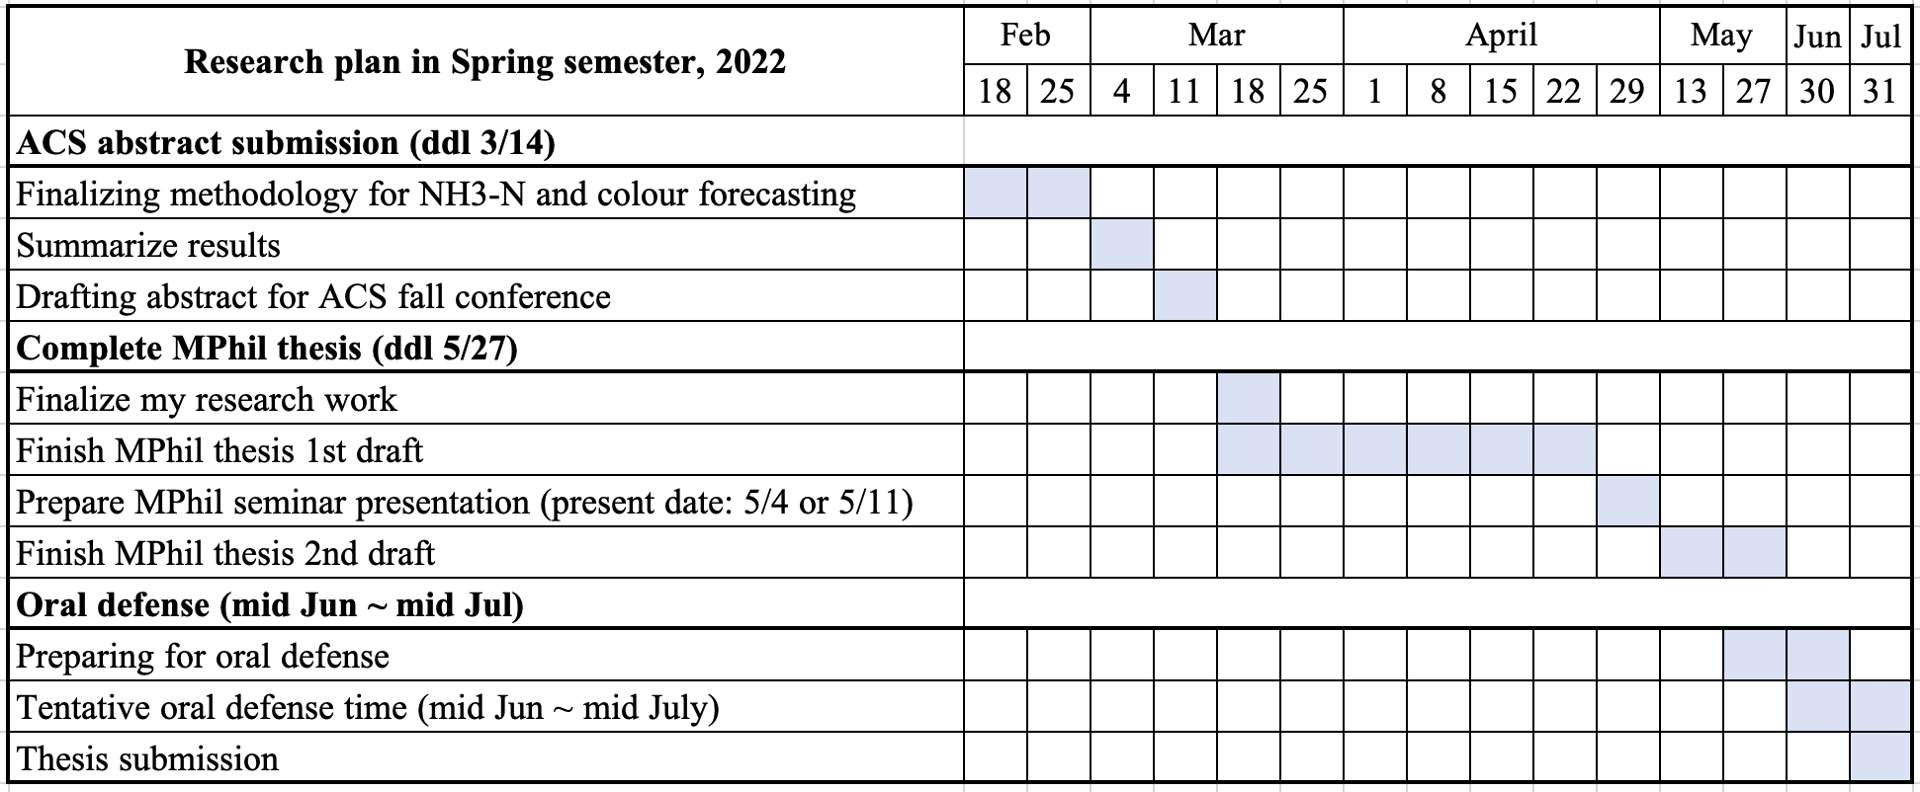
\includegraphics{/Users/tinghsi/OneDrive - HKUST Connect/MPhil-thesis-github-library/MPhil-thesis/Presentation-notes/0314-progress-report/plan.png}
\caption{plan}
\end{figure}

\hypertarget{progress-report}{%
\subsection{Progress report}\label{progress-report}}

\textbf{Key findings in Feb and March}\\
1. Train ammonia forecasting model with colour decreased the model
performance.\\
2. New method was used to increase the model training data quality
(i.e., feature engineering).\\
3. New state-of-the-art model (Transformer) is used and a better model
performance is achieved compared to LSTM and DNN.

\end{document}
